\documentclass{beamer}
%
% Choose how your presentation looks.
%
% For more themes, color themes and font themes, see:
% http://deic.uab.es/~iblanes/beamer_gallery/index_by_theme.html
%
\mode<presentation>
{
  \usetheme{default}      % or try Darmstadt, Madrid, Warsaw, ...
  \usecolortheme{default} % or try albatross, beaver, crane, ...
  \usefonttheme{default}  % or try serif, structurebold, ...
  \setbeamertemplate{navigation symbols}{}
  \setbeamertemplate{caption}[numbered]
} 

\usepackage[english]{babel}
\usepackage[utf8x]{inputenc}
\usepackage{amsmath,amsfonts}
\usepackage{tikz}

\title[Your Short Title]{Probabilidade e Estatística}
\author{José William Vitorino de Souza}
\institute{IFCE - Aracati}
\date{27/03/2018}

\begin{document}

\begin{frame}
  \titlepage
\end{frame}

 %Uncomment these lines for an automatically generated outline.
%\begin{frame}{Outline}
  %\tableofcontents
%\end{frame}

\section{Some \LaTeX{} Examples}

\subsection{Modelo de Bernoulli}

\begin{frame}{Modelo de Bernoulli}

Dizemos que uma variável X segue o modelo Bernoulli se atribui 0 ou 1 à ocorrência de fracasso ou sucesso, respectivamente. Com \textit{p} representando probabilidade de sucesso, \[ 0 \leq \textit{p} \] \[ \textit{p} \leq 1 \] Sua função discreta de probabilidade é por:

\begin{table}[]
\centering
\label{my-label}
\begin{tabular}{l|ll}
X & 0 & 1 \\ \hline
\textit{Pi} & \textit{1 - p} & \textit{p}
\end{tabular}
\end{table}

Ou de modo resumido P( X = \textit{x} ) = \( p^x \) \( (1 - p)^{1-x} \), x = 0,1.

\end{frame}

\begin{frame}{Exemplo}

Sabe-se que a eficiência de ume vacina é de 80\%. Um grupo de três indivíduos é sorteado, dentre a população vacinada, e submetido a testes para averiguar se a imunização foi efetiva, evento representado por \textit{I}. A árvore
probabilidades é apresen tada a seguir:

\centering
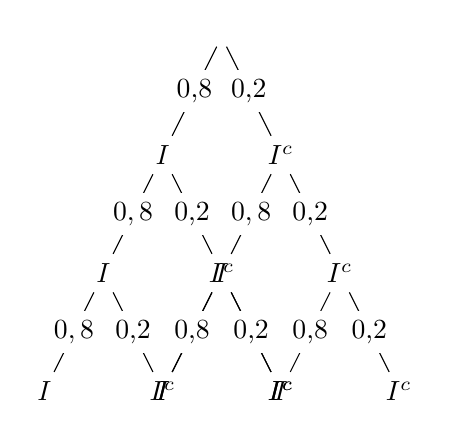
\begin{tikzpicture}
%	\tikzstyle{level 1} = [level distance=1cm]
%	\tikzstyle{level 2} = [level distance=1cm]
%	\tikzstyle{level 3} = [level distance=1cm]
	\node{}
		child{
			node{\textit{I}}
				child{
					node{\textit{I}}
						child{
							node{\textit{I}}
							edge from parent
							node[fill=white]{\(0,8\)}
						}
						child{
							node{\textit{\( I^c \)}}
							edge from parent
							node[fill=white]{0,2}
						}
					edge from parent
					node[fill=white]{\(0,8\)}
				}
				child{
					node{\textit{\( I^c \)} }
						child{
							node{\textit{I}}
							edge from parent
							node[fill=white]{0,8}
						}
						child{
							node{\textit{\( I^c \)}}
							edge from parent
							node[fill=white]{0,2}
						}
					edge from parent
					node[fill=white]{0,2}
				}
			edge from parent
			node[fill=white]{0,8}
		}
		child{
			node{\textit{\( I^c \)}   }
				child{
					node{\textit{I}}
						child{
							node{\textit{I}}
							edge from parent
							node[fill=white]{0,8}
						}
						child{
							node{\textit{\( I^c \)}}
							edge from parent
							node[fill=white]{0,2}
						}
					edge from parent
					node[fill=white]{\(0,8\)}
				}
				child{
					node{\textit{\( I^c \)}}
						child{
							node{\textit{I}}
							edge from parent
							node[fill=white]{0,8}
						}
						child{
							node{\textit{\( I^c \)}}
							edge from parent
							node[fill=white]{0,2}
						}
					edge from parent
					node[fill=white]{0,2}
				}
			edge from parent
			node[fill=white]{0,2}
		};

\end{tikzpicture}

\end{frame}

\begin{frame}{Tabela}

A variável X(número de indivíduos imunizados), assume os valores 0, 1, 2, e 3 com probabilidades calculadas com o auxílio da árvore e apresentadas na tabela:

\begin{table}[]
\centering
\label{tablex}
\begin{tabular}{|l|l|l|}
\hline
Eventos                                                                     & Probabilidade                         & X \\ \hline
III                                                                         & \( 0,8^3 \)           & 3 \\ \hline
II\( I^c \)                                                 & \( 0,8^2 \)x 0,2      & 2 \\ \hline
I\( I^c \)I                                                 & \( 0,8^2 \)x 0,2      & 2 \\ \hline
I\( I^c \)\( I^c \)                         & \( 0,8 \)x\( 0,2^2 \) & 1 \\ \hline
\( I^c \)II                                                 & \( 0,8^2 \)x 0,2      & 2 \\ \hline
\( I^c \)I\( I^c \)                         & \( 0,8 \)x\( 0,2^2 \) & 1 \\ \hline
\( I^c \)\( I^c \)I                         & \( 0,8 \)x\( 0,2^2 \) & 1 \\ \hline
\( I^c \)\( I^c \)\( I^c \) & \( 0,2^3 \)           & 0 \\ \hline
\end{tabular}
\end{table}
\end{frame}

\begin{frame}{Função de probabilidade}

Função de probabilidade:

\begin{table}[]
\centering
\label{funcaoprobabilidade}
\begin{tabular}{l|llll}
X  & 0                         & 1                                   & 2                                       & 3                         \\ \hline
Pi & /(0,2^3/) & 3 x 0,8 x /(0,2^2/) & 3 x /(0,8^2/) x 0,2 & /(0,8^3/)
\end{tabular}
\end{table}
\end{frame}

\end{document}
